\chapter{A Type 2 Asymmetric ASA on Symmetric Encryption} \label{sec:asymASA2}

In the last chapter, we presented a type 1 asymmetric ASA, where no other parties besides the subverter, even if they have the embedded key $ek$, would be able to detect the subversion. In this chapter we will explore a more nuanced requirement of undetectability. In fact, we will present an asymmetric ASA that is \emph{detectable} in the augmented detectability game in \autoref{game:gendetect}, but undetectable in the regular detectability game. This is a type 2 asymmetric ASA.

To see why such an ASA may still be relevant, consider again the context of an ASA. There are three relevant parties: the subverter, the user $\mathcal{U}$, and some third party $\mathcal{V}$. The subverter is executing an algorithm substitution attack on $\mathcal{U}$. It is critically important that $\mathcal{U}$ is not able to detect the ASA, since then $\mathcal{U}$ will stop using the subverted scheme. The subverter relies on the fact the $\mathcal{U}$ is not able to examine the code being used. Hence the situations in which $\mathcal{U}$ knows the embedded key $ek$, but does not already know of the subversion, are limited. With this reasoning, we can restrict ourselves to evaluating the detectability of an ASA with respect to a user $\mathcal{U}$ only in the regular detectability game, regardless of whether or not the ASA is symmetric or asymmetric.

On the other hand, the requirements on the third party $\mathcal{V}$ are different, and for a type 2 asymmetric ASA we will allow for the possibility that a sophisticated third party $\mathcal{V}$ is able to reverse-engineer the cryptographic scheme and obtain the key $ek$ or outright detect the scheme in this way. Such a $\mathcal{V}$ may not have decision-making authority to change the scheme being used, so it may not be catastrophic for $\mathcal{V}$ to be able to detect the ASA. Hence requiring augmented undetectability with respect to $\mathcal{V}$ is not necessary. The real requirement for a type 2 asymmetric ASA is that the subverter is the only one able to take advantage of the subversion and break the security of the subverted scheme. To reflect this, we can simply require that the subverted algorithm $\mathsf{ASub.Alg_\lambda}$ preserve security properties of the original algorithm $\mathsf{\Lambda.Alg_\lambda}$.\footnote{A version of security preservation appears in Appendix A of the eprint version of \cite{FSE:DegFarPoe15}. The authors obtained an elegant result relating the security of a subverted scheme to the security of the original scheme and the detectability of the ASA by an adversary who is in possession of the key $\overline{k}$. However, they only considered symmetric ASAs; the asymmetric case is certainly different.}

The situation described above admittedly has stronger behavioural assumptions on the involved parties than the one we covered in \autoref{sec:asymASA}, where we proved that even $\mathcal{V}$ would not be able to detect the subversion. The reason that we wish to consider this more restricted context is that we will be able to construct a type 2 asymmetric ASA (one that satisfies the above notion of undetectability) that is less susceptible to detection via timing side channels. We will still use a repetition parameter $s$ in the same way as in the ASA from \autoref{sec:asymASA}, but key recovery will be possible with a smaller $s$.

Before continuing, we will define the notions of IND-CPA security for symmetric and asymmetric encryption. This is a weaker form of security than IND\$ we used in \autoref{sec:asymASA} (which implicitly was in chosen-plaintext form), but it is all we will require in this chapter.

The IND-CPA games for symmetric encryption scheme $\mathsf{SE}$ and public-key encryption scheme $\mathsf{PKE}$ are given in \autoref{game:indpke}.

The advantage of $\mathcal{B}$ at each of these games is
\shortlongeqn[]{
\text{Adv}^{\mathrm{IND}\text{-}\mathrm{CPA}}_\mathsf{PKE}(\mathcal{B})=\lvert \prob{\mathrm{IND}\text{-}\mathrm{CPA}_\mathsf{PKE}(\mathcal{B})}-\frac{1}{2} \rvert
}
and
\shortlongeqn[.]{
\text{Adv}^{\mathrm{IND}\text{-}\mathrm{CPA}}_\mathsf{SE}(\mathcal{B})=\lvert \prob{\mathrm{IND}\text{-}\mathrm{CPA}_\mathsf{SE}(\mathcal{B})}-\frac{1}{2} \rvert
}
Informally, we say that the schemes $\mathsf{PKE}$ and $\mathsf{SE}$ are IND-CPA-secure if the advantage of any efficient adversary $\mathcal{B}$ in the corresponding game is small.

\begin{figure}
\centering
\begin{pchstack}
\myprocedure[linenumbering]{IND-CPA$_{\mathsf{SE}}(\mathcal{B})$}{
	k \sample \mathsf{SE.KeyGen()} \\
	b \sample \{0,1\} \\
	b' \sample \mathcal{B}^{\mathcal{O}_\mathsf{SE.Enc}} \\
	\pcreturn b=b'
}
\myprocedure[linenumbering]{$\mathcal{O}_\mathsf{SE.Enc}(m)$}{
	\pcif b=0 \pcthen \\
	\pcind c \sample \mathsf{SE.Enc}(k,m) \\
	\pcif b=1 \pcthen \\
	\pcind c \sample \mathsf{SE.Enc}(k,\mathbf{0}) \\
	\pcreturn c
}
\vrule\
\myprocedure[linenumbering]{IND-CPA$_{\mathsf{PKE}}(\mathcal{B})$}{
	(pk, sk) \sample \mathsf{PKE.KeyGen()} \\
	b \sample \{0,1\} \\
	b' \sample \mathcal{B}^{\mathcal{O}_\mathsf{PKE.Enc}}(pk) \\
	\pcreturn b=b'
}
\myprocedure[linenumbering]{$\mathcal{O}_\mathsf{PKE.Enc}(m)$}{
	\pcif b=0 \pcthen \\
	\pcind c \sample \mathsf{PKE.Enc}(pk,m) \\
	\pcif b=1 \pcthen \\
	\pcind c \sample \mathsf{PKE.Enc}(pk,\mathbf{0}) \\
	\pcreturn c
}
\end{pchstack}
\caption[The IND-CPA games for a symmetric encryption scheme $\mathsf{SE}$ and a public-key encryption scheme $\mathsf{PKE}$]{The IND-CPA games for (left) a symmetric encryption scheme $\mathsf{SE}$ and (right) a public-key encryption scheme $\mathsf{PKE}$.}
\label{game:indse}
\label{game:indpke}
\end{figure}

We use a ``multi-challenge'' IND-CPA game, where $\mathcal{B}$ is not limited to a single challenge ciphertext from which it has to guess. This multi-challenge game has been used, for example, by Rogaway \cite{FSE:Rogaway04}. We choose to use this particular notion, as it more closely resembles our detectability games, leading to proofs that are easier to follow. Security of multi-challenge IND-CPA follows from single-challenge security using a hybrid argument.

We now present our type 2 asymmetric ASA $\mathsf{ASub2}$. Let $\mathsf{SE}$ be a symmetric encryption scheme. Let $\mathsf{PKE}$ be an IND-CPA-secure public-key encryption scheme, and let $\mathsf{F}$ be a PRF with output space $\{1,...,\mathsf{PKE.clen}\}\times \{0,1\}$. Then $\mathsf{ASub2}$, an ASA on $\mathsf{SE}$ is shown in \autoref{figure:asymsubv2}, where $s$ is a parameter of the subversion to bound the loops as before.

\begin{wrapfigure}{R}{0.4\textwidth}
\centering
\myprocedure[linenumbering]{$\textsf{ASub2.Enc}(k,m,ek,\tau)$}{
	\pcif \tau = \bot \pcthen \\
	\pcind \kappa \sample \textsf{PKE.Enc}(ek, k); \tau \leftarrow \kappa \\
	\pcelse \kappa \leftarrow \tau \\
	j \leftarrow 0 \\
	\textbf{do} \\
	\pcind j \leftarrow j + 1 \\
	\pcind r \sample \{0,1\}^\mathsf{SE.rlen} \\
	\pcind c \leftarrow \mathsf{SE.Enc}(k, m; r) \\
	\pcind (\sigma, w) \leftarrow \mathsf{F}(ek, c) \\
	\pcuntil \kappa[\sigma] = w \textbf{ or } j = s \\
	\pcreturn (c, \tau)
}
\caption[Type 2 asymmetric ASA on symmetric encryption]{Type 2 asymmetric ASA on symmetric encryption.}
\label{figure:asymsubv2}
\end{wrapfigure}

The function $\mathsf{ASub2.Enc}$ bears many similarities to $\mathsf{ASub.Enc}$ from \autoref{sec:asymASA} and to the ASA of \cite{CCS:BelJaeKan15}. In fact, the ASA $\mathsf{ASub}$ essentially consists of encrypting $k$ to $\kappa$ using IND\$-secure public-key encryption, and then leaking $\kappa$ using the same techniques as \cite{C:BelPatRog14}. The ASA $\mathsf{ASub2}$, on the other hand, consists of encrypting $k$ to $\kappa$ using IND-CPA-secure public-key encryption, and then leaking $\kappa$ using the same techniques as \cite{CCS:BelJaeKan15}. We will explore some of these parallels in \autoref{sec:generalize}.

The fundamental difference between the two ASAs $\mathsf{ASub}$ and $\mathsf{ASub2}$, as well as the reason for no longer requiring $\mathsf{PKE}$ to be IND\$, becomes evident when we consider how an adversary $\mathcal{V}$ in possession of the key $ek$ is able to interact with the scheme. Informally, the subverter is able to obtain $k$ because anyone with $ek$ can obtain $\kappa$, and the subverter can obtain $k$ from $\kappa$ using $xk$. In the case of $\mathsf{ASub}$, we required $\mathsf{PKE}$ to be IND\$ so that the adversary $\mathcal{V}$ would not be able to distinguish the $\kappa$ they obtain by this process from random bits. Making sure to never leak the same bit of $\kappa$ twice, we proved that this makes the scheme undetectable. For the ASA $\mathsf{ASub2}$, even an IND\$ scheme would not provide this guarantee. Re-use of the same $\kappa$ for more than $|\kappa|$ encryptions is required: randomization of the leaked bit of $\kappa$ on each execution means that $\mathcal{V}$ cannot be sure all have been leaked. Therefore all (index, bit)-pairs that $\mathcal{V}$ receives using this decoding process that have the same index will also have the same bit with certainty, and this is unlikely in an unsubverted scheme. While not undetectable, we can still show that the subverted scheme is secure against $\mathcal{V}$, implying that $\mathcal{V}$ is not able to recover the secret key in the same way as the subverter.

In the rest of this chapter, we will prove that $\mathsf{ASub2}$ is a type 2 asymmetric ASA. That is, we will prove that the scheme is (1) undetectable to the user $\mathcal{U}$ in the regular detection game, (2) secure against the third party $\mathcal{V}$, and (3) that the subverter can recover the secret key $k$.

\section{Undetectability of our type 2 asymmetric ASA}
We first prove undetectability of $\mathsf{ASub2}$ against an adversary $\mathcal{U}$ in the regular state reset detectability game SRDET.

\begin{theorem} \label{theorem:detect2}
Let $\mathcal{U}$ be an adversary in the regular state reset detectability game in \autoref{game:gendetect}, $\mathrm{SRDET}_\mathsf{ASub2}(\mathcal{U})$, with symmetric encryption scheme $\mathsf{SE}$ as $\mathsf{\Lambda}$ and $\mathsf{SE.Enc}$ as $\mathsf{\Lambda.Alg}_\lambda$, where $\mathsf{ASub2.Enc}$ is the algorithm given in \autoref{figure:asymsubv2}. If $n$ is the number of queries that $\mathcal{U}$ makes to its encryption oracle, and $\eta$ is the min-entropy of $\mathsf{SE.Enc}$, then there is an adversary $\mathcal{F}$ against the $\mathrm{PRF}$-security of $\mathsf{F}$ such that
\shortlongeqn[.]{
\mathrm{Adv}^{\mathrm{SRDET}}_{\mathsf{ASub}}(\mathcal{U}) \leq 
2\mathrm{Adv}^{\mathrm{PRF}}_{\mathsf{F}}(\mathcal{F})
+ (ns)^2\cdot 2^{-\eta-1}
}
The running time of $\mathcal{F}$ is about that of $\mathcal{U}$, and $\mathcal{F}$ makes at most $ns$ oracle queries.
\end{theorem}
\begin{proof}
We proceed by a sequence of games. Let $I_0$ the regular state reset detectability game of \autoref{game:gendetect}, with all the substitutions in the theorem statement. Let $I_1$ be the same as $I_0$ but with $\mathsf{F}$ replaced by lazy random sampling; this is given in \autoref{game:I12}. Let $I_2$ be the same as $I_1$ but with $w$ and $\sigma$ sampled randomly instead; this is also given in \autoref{game:I12}. Let $I_3$ be the regular state reset detectability game where the encryption oracle is replaced by an oracle that simply returns $\mathsf{SE.Enc}(k,m)$, and the $\mathsf{Reset}$ oracle removed.

\begin{figure}
\centering
\begin{pchstack}
\begin{pcvstack}
\myprocedure[linenumbering]{$I_{1/2}(\mathcal{U})$}{
	(ek, xk) \sample \mathsf{ASub2.KeyGen()}\\
	C \leftarrow \emptyset \\
	i \leftarrow 1 \\
	\tau_0 \leftarrow \bot \\
	b \sample \{0,1\} \\
	b' \sample \mathcal{U}^{\mathcal{O}_\mathsf{Enc},\mathsf{Reset}} \\
	\pcreturn b=b'
}
\pcvspace
\myprocedure[linenumbering]{$\mathsf{Reset}(j)$, \hfill $0\le j<i$}{
	\pcif b = 1 \pcthen \\
	\pcind \tau_{i} \leftarrow \tau_{j} \\
	\pcind i \leftarrow i + 1
}
\pcvspace
\myprocedure[linenumbering]{$\mathcal{O}_\mathsf{Enc}(k,m)$}{
	\pcif b=0 \pcthen c \sample \mathsf{Enc}(k,m) \\
	\pcif b=1 \pcthen \\
	\pcind (c, \tau_i) \sample \mathsf{Helper}(k,m,ek,\tau_{i-1}) \\
	\pcind i \leftarrow i + 1 \\
	\pcreturn c
}
\end{pcvstack}
\pchspace
\myprocedure[linenumbering]{$\mathsf{Helper}(k,m,ek,\tau)$}{
	\pcif \tau = \bot \pcthen \\
	\pcind \kappa \sample \textsf{PKE.Enc}(ek, k); \tau \leftarrow \kappa \\
	\pcelse \kappa \leftarrow \tau \\
	j \leftarrow 0 \\
	\textbf{do} \\
	\pcind j \leftarrow j + 1 \\
	\pcind r \sample \{0,1\}^\mathsf{SE.rlen} \\
	\pcind c \leftarrow \mathsf{SE.Enc}(k, m; r) \\
	\pcind \pcbox{\pcif c \notin C \pcthen} \\
	\pcind \pcind (\sigma_c, w_c) \sample \{0,...,\mathsf{PKE.clen}\}\times \{0,1\} \\
	\pcind \pcind C \leftarrow C\cup \{c\} \\
	\pcind \pcbox{\pcelse \mathsf{bad} \leftarrow \mathsf{true}} \\
	\pcind \sigma,w \leftarrow \sigma_c,w_c \\
	\pcuntil \kappa[\sigma] = w \textbf{ or } j = s \\
	\pcreturn (c, \tau)
}
\end{pchstack}
\caption[Games $I_1$ and $I_2$ for the proof of \autoref{theorem:detect2}]{Games $I_1$ and $I_2$ for the proof of \autoref{theorem:detect2}. Game $I_1$ contains the boxed code while game $I_2$ does not (including the appropriate indentation corrections).}
\label{game:I12}
\end{figure}

Consider first games $I_0$ and $I_1$. Similarly to the proof of \autoref{theorem:detect2}, this is a straightforward gamehop based on indistinguishability of the PRF $\mathsf{F}$, so we omit the detailed reduction.  Instead, note that an adversary $\mathcal{F}$ in the $\mathrm{PRF}_\mathsf{F}(\mathcal{F})$ game is able to completely simulate the games $I_0$ and $I_1$ for an adversary $\mathcal{U}$ using the oracle provided to it in place of $\mathsf{F}$. Let $b_\mathrm{PRF}$ be the challenge bit in the PRF game. Then if $b_\mathrm{PRF}=1$, the $\mathsf{Enc}$ oracle simulated by $\mathcal{F}$ proceeds exactly as in game $I_1$, and if  $b_\mathrm{PRF}=0$, then it proceeds exactly as in game $I_0$. Thus we have
\shortlongeqn[,]{
\condprob{\mathcal{F} \Rightarrow 1}{b_\mathrm{PRF} = 1} = \prob{I_1}
}
\shortlongeqn[,]{
\condprob{\mathcal{F} \Rightarrow 1}{b_\mathrm{PRF} = 0} = \prob{I_0}
}
and hence
\shortlongeqn[.]{
|\prob{I_1}-\prob{I_0}| = 2\text{Adv}^{\mathrm{PRF}}_\mathsf{PKE}(\mathcal{F})
}

Now consider games $I_1$ and $I_2$. In game $I_2$, we replace the selection of $w$ and $\sigma$ in the encryption oracle with true random sampling of $w$ and $\sigma$, regardless of whether $c$ was input to the random oracle before. Let $\mathsf{Col}$ be the event where $\mathsf{bad}$ is set to $\mathsf{true}$ in game $I_2$. This happens when some $c$ previously generated by the encryption oracle is obtained again during an encryption oracle query. We upper bound $\prob{\mathsf{Col}}$: let $\eta$ be the min-entropy of $\mathsf{SE.Enc}$. Then we have that
\shortlongeqn[.]{
\prob{\mathsf{Col}} \le \binom{ns}{2}\cdot 2^{-\eta} \le (ns)^2\cdot 2^{-\eta-1}
}

By the Fundamental Lemma of Game-Playing \cite{EC:BelRog06}, we have
\shortlongeqn[.]{
|\prob{I_2}-\prob{I_1}| \le \prob{\mathsf{Col}} \le (ns)^2\cdot 2^{-\eta-1}
}

Finally, $I_3$ was defined as the detectability game where the encryption oracle is replaced by an oracle that simply returns $\mathsf{SE.Enc}(k,m)$. In game $I_2$, since the loop condition is no longer dependent on the selection of $c$, the implementation $\mathsf{ASub2.Enc}_2$ is identical to $\mathsf{SE.Enc}(k,m)$. Hence $\prob{I_2}=\prob{I_3}$. Further, note that $\prob{I_3}=\frac{1}{2}$, since the encryption oracle in $I_3$ is not dependent on $b$.

Putting all these results together, we have
\iffullversion
\begin{align*}
\text{Adv}^\text{SRDET}_\mathsf{ASub2}(\mathcal{U})
&= |\prob{I_0}-\frac{1}{2}| \\
&= |\prob{I_0}-\prob{I_1}+\prob{I_1}-\prob{I_2}+\prob{I_2}-\frac{1}{2}| \\
&\le |\prob{I_0}-\prob{I_1}|+|\prob{I_1}-\prob{I_2}|+|\prob{I_2}-\frac{1}{2}| \\
&\le 2\text{Adv}^{\text{PRF}}_\mathsf{F}(\mathcal{F}) + (ns)^2\cdot 2^{-\eta-1} + |\prob{I_3}-\frac{1}{2}| \\
&= 2\text{Adv}^{\text{PRF}}_\mathsf{F}(\mathcal{F}) + (ns)^2\cdot 2^{-\eta-1},
\end{align*}
\else
\[
\text{Adv}^\text{SRDET}_\mathsf{ASub2}(\mathcal{U}) \le 2\text{Adv}^{\text{PRF}}_\mathsf{F}(\mathcal{F}) + (ns)^2\cdot 2^{-\eta-1},
\]
\fi
as desired.

\end{proof}

\section{Security of our type 2 asymmetric ASA} \label{sec:security}
We prove here that the ASA $\mathsf{ASub2}$ is secure against an adversary $\mathcal{V}$ who has knowledge of $ek$. ``Secure'', here, should mean in the same sense as the original symmetric encryption scheme: IND-CPA. However, we cannot apply this notion directly to $\mathsf{ASub2}$, since the IND-CPA game does not provide the necessary parameters. Instead, we introduce the modified game IND-CPA$'$ on $\mathsf{ASub2}$ with adversary $\mathcal{V}$, shown in \autoref{game:ind'}. This game contains the required modifications to \autoref{game:indse} in order to include the function $\mathsf{ASub2.Enc}$, as well as providing the embedded key $ek$ to the adversary $\mathcal{V}$. Assuming that $\mathsf{SE.Enc}$ is IND-CPA secure, we say that $\mathsf{ASub2.Enc}$ is secure if it is IND-CPA$'$ secure against $\mathcal{V}$.

\begin{figure}
\centering
\begin{pchstack}
\myprocedure[linenumbering]{IND-CPA$'_{\mathsf{ASub2}}(\mathcal{V})$}{
	(ek, xk) \sample \mathsf{ASub2.KeyGen()} \\
	k \sample \mathsf{SE.KeyGen()} \\
	\tau \leftarrow \bot \\
	b \sample \{0,1\} \\
	b' \sample \mathcal{V}^{\mathcal{O}_\mathsf{ASub2.Enc}}(ek) \\
	\pcreturn b=b'
}
\pchspace
\myprocedure[linenumbering]{$\mathcal{O}_\mathsf{ASub2.Enc}(m)$}{
	\pcif b=0 \pcthen \\
	\pcind (c, \tau) \sample \mathsf{ASub2.Enc}(k,m,ek,\tau) \\
	\pcif b=1 \pcthen \\
	\pcind (c, \tau) \sample \mathsf{ASub2.Enc}(k,\mathbf{0},ek,\tau) \\
	\pcreturn c
}
\end{pchstack}
\caption[The IND-CPA$'$ game for asymmetric ASA $\mathsf{ASub2}$]{The IND-CPA$'$ game for asymmetric ASA $\mathsf{ASub2}$.}
\label{game:ind'}
\end{figure}

\begin{theorem} \label{theorem:security}
Let $\mathsf{SE}$ be a symmetric encryption scheme, and let $\mathsf{ASub2}$ be the ASA on $\mathsf{SE}$ given by the description in \autoref{figure:asymsubv2}. Let $\mathcal{V}$ be an adversary in the game $\mathrm{IND}\text{-}\mathrm{CPA}'_{\mathsf{ASub2.Enc}}(\mathcal{V})$. Then there is an adversary $\mathcal{B}_1$ against the $\mathrm{IND}$-$\mathrm{CPA}$ security of $\mathsf{PKE}$ and an adversary $\mathcal{B}_2$ against the $\mathrm{IND}$-$\mathrm{CPA}$ security of $\mathsf{SE}$ such that
\shortlongeqn[.]{
\mathrm{Adv}^{\mathrm{IND}\text{-}\mathrm{CPA}'}_{\mathsf{ASub2}}(\mathcal{V}) \leq 
2\mathrm{Adv}^{\mathrm{IND}\text{-}\mathrm{CPA}}_{\mathsf{PKE}}(\mathcal{B}_1)
+ 2\mathrm{Adv}^{\mathrm{IND}\text{-}\mathrm{CPA}}_{\mathsf{SE}}(\mathcal{B}_2)
}
The running time of $\mathcal{B}_1$ and $\mathcal{B}_2$ are both about that of $\mathcal{V}$. If $n$ is the number of oracle queries that $\mathcal{V}$ makes, then $\mathcal{B}_1$ makes $n$ queries to its own oracle, and $\mathcal{B}_2$ makes at most $ns$ queries to its own oracle.
\end{theorem}
\begin{proof}

We proceed by a sequence of games. Let $J_0$ be the $\mathrm{IND}\text{-}\mathrm{CPA}'_{\mathsf{ASub2.Enc}}(\mathcal{V})$ game. Let $J_1$ be the same as $J_0$ but with $\kappa$ computed as an encryption of $\mathbf{0}$ instead of as an encryption of $k$. Let $J_2$ be the same as $J_1$ but with $c$ computed as an encryption of $\mathbf{0}$ instead of as an encryption of $m$. All of these games are shown in \autoref{game:J012B12}.

Let $\mathcal{B}_1$, defined in \autoref{game:J012B12}, be an adversary to the IND-CPA game on $\mathsf{PKE}$. Acting as a challenger, $\mathcal{B}_1$ simulates the IND-CPA game on $\mathsf{ASub2}$ for $\mathcal{V}$, in particular using the $\mathsf{PKE.Enc}$ oracle and public key given to it to simulate $\mathsf{ASub2.Enc}$.

\begin{figure}[t]
\centering
\begin{pchstack}
\begin{pcvstack}
\myprocedure[linenumbering]{$J_{0,1,2}(\mathcal{V})$}{
	(ek, xk) \sample \mathsf{ASub2.KeyGen()} \\
	k \sample \mathsf{SE.KeyGen()}\\
	\tau \leftarrow \bot \\
	b \sample \{0,1\} \\
	b' \sample \mathcal{V}^{\mathcal{O}_\mathsf{Enc}}(ek) \\
	\pcreturn b=b'
}
\pcvspace
\myprocedure[linenumbering]{$\mathcal{O}_\mathsf{Enc}(m)$}{
	\pcif b=0 \pcthen \\
	\pcind (c, \tau) \sample \mathsf{Helper}(k,m,ek,\tau) \\
	\pcif b=1 \pcthen \\
	\pcind (c, \tau) \sample \mathsf{Helper}(k,\mathbf{0},ek,\tau) \\
	\pcreturn c
}
\pcvspace
\myprocedure[linenumbering]{$\mathsf{Helper}(k,m,ek,\tau)$}{
	\pcif \tau = \bot \pcthen \\
	\pcind \pcbox{\kappa \sample \textsf{PKE.Enc}(ek, k)}_0 \\
	\pcind \pcbox{\kappa \sample \textsf{PKE.Enc}(ek, \mathbf{0})}_{1,2} \\
	\pcind \tau \leftarrow \kappa \\
	\pcelse \kappa \leftarrow \tau \\
	j \leftarrow 0 \\
	\textbf{do} \\
	\pcind j \leftarrow j + 1 \\
	\pcind r \sample \{0,1\}^\mathsf{SE.rlen} \\
	\pcind \pcbox{c \leftarrow \mathsf{SE.Enc}(k, m; r)}_{0,1} \\
	\pcind \pcbox{c \leftarrow \mathsf{SE.Enc}(k, \bf{0}; r)}_{2} \\
	\pcind (\sigma, w) \leftarrow \mathsf{F}(ek, c) \\
	\pcuntil \kappa[\sigma] = w \textbf{ or } j = s \\
	\pcreturn (c, \tau)
}
\end{pcvstack}
\pchspace
\unskip\ \vrule\
\begin{pcvstack}
\myprocedure[linenumbering]{$\mathcal{B}_1^{\mathcal{O}_\mathsf{PKE.Enc}}(pk)$}{
	k \sample \mathsf{SE.KeyGen()} \\
	\tau \leftarrow \bot \\
	b_\text{1} \sample \{0,1\} \\
	b_\text{1}' \sample \mathcal{V}^{\mathcal{O}_\mathsf{Enc}}(pk) \\
	\pcif b_\text{1}=b_\text{1}'\ \pcreturn 1 \\
	\pcelse \pcreturn 0
}
\pcvspace
\myprocedure[linenumbering]{$\mathcal{O}_\mathsf{Enc}(m)$}{
	\pcif b_\text{1}=0 \pcthen \\
	\pcind (c, \tau) \sample \mathsf{Helper}(k,m,pk,\tau) \\
	\pcif b_\text{1}=1 \pcthen \\
	\pcind (c, \tau) \sample \mathsf{Helper}(k,\mathbf{0},pk,\tau) \\
	\pcreturn c
}
\pcvspace
\myprocedure[linenumbering]{$\mathsf{Helper}(k,m,pk,\tau)$}{
	\pcif \tau = \bot \pcthen \\
	\pcind \pcbox{\kappa \sample \mathcal{O}_\mathsf{PKE.Enc}(k)} \\
	\pcind \tau \leftarrow \kappa \\
	\pcelse \kappa \leftarrow \tau \\
	j \leftarrow 0 \\
	\textbf{do} \\
	\pcind j \leftarrow j + 1 \\
	\pcind r \sample \{0,1\}^\mathsf{SE.rlen} \\
	\pcind c \leftarrow \mathsf{SE.Enc}(k, m; r) \\
	\pcind (\sigma, w) \leftarrow \mathsf{F}(\pcbox{pk}, c) \\
	\pcuntil \kappa[\sigma] = w \textbf{ or } j = s \\
	\pcreturn (c, \tau)
}
\end{pcvstack}
\pchspace
\unskip\ \vrule\
\begin{pcvstack}
\myprocedure[linenumbering]{$\mathcal{B}_2^{\mathcal{O}_\mathsf{SE.Enc}}$}{
	(ek, xk) \sample \mathsf{PKE.KeyGen()} \\
	\tau \leftarrow \bot \\
	b_\text{2} \sample \{0,1\} \\
	b_\text{2}' \sample \mathcal{V}^{\mathcal{O}_\mathsf{Enc}}(ek) \\
	\pcif b_\text{2}=b_\text{2}'\ \pcreturn 1 \\
	\pcelse \pcreturn 0
}
\pcvspace
\myprocedure[linenumbering]{$\mathcal{O}_\mathsf{Enc}(m)$}{
	\pcif b_\text{2}=0 \pcthen \\
	\pcind (c, \tau) \sample \mathsf{Helper}(k,m,ek,\tau) \\
	\pcif b_\text{2}=1 \pcthen \\
	\pcind (c, \tau) \sample \mathsf{Helper}(k,\mathbf{0},ek,\tau) \\
	\pcreturn c
}
\pcvspace
\myprocedure[linenumbering]{$\mathsf{Helper}(k,m,ek,\tau)$}{
	\pcif \tau = \bot \pcthen \\
	\pcind \kappa \sample \textsf{PKE.Enc}(ek, \mathbf{0}) \\
	\pcind \tau \leftarrow \kappa \\
	\pcelse \kappa \leftarrow \tau \\
	j \leftarrow 0 \\
	\textbf{do} \\
	\pcind j \leftarrow j + 1 \\
	\pcind \pcbox{c \leftarrow \mathcal{O}_\mathsf{SE.Enc}(m)} \\
	\pcind (\sigma, w) \leftarrow \mathsf{F}(ek, c) \\
	\pcuntil \kappa[\sigma] = w \textbf{ or } j = s \\
	\pcreturn (c, \tau)
}
\end{pcvstack}
\end{pchstack}
\caption[Games $J_0,J_1,$ and $J_2$ and adversaries $\mathcal{B}_1$ and $\mathcal{B}_2$ for proof of \autoref{theorem:security}]{Games $J_0,J_1,$ and $J_2$ and adversaries $\mathcal{B}_1$ and $\mathcal{B}_2$ for proof of \autoref{theorem:security}. In the $J$-games, each game only include the boxed code if it has matching subscript. In $\mathcal{B}_1$ and $\mathcal{B}_2$, the boxes serve to highlight changes.}
\label{game:J012B12}
\end{figure}

Let $b_\text{pke}$ denote the bit from the IND-CPA$_\mathsf{PKE}(\mathcal{B}_1)$ game. Note that if $b_{pke}=1$, then the $\mathsf{Enc}$ oracle simulated by $\mathcal{B}_1$ proceeds exactly as in game $J_1$, and if $b_{pke}=0$, then it proceeds exactly as in game $J_0$. Thus we have
\shortlongeqn[,]{
\condprob{\mathcal{B}_1 \Rightarrow 1}{b_{pke} = 1} = \prob{J_1}
}
\shortlongeqn[,]{
\condprob{\mathcal{B}_1 \Rightarrow 1}{b_{pke} = 0} = \prob{J_0}
}
and hence
\shortlongeqn[.]{
|\prob{J_1}-\prob{J_0}| = 2\text{Adv}^{\text{IND-CPA}}_\mathsf{PKE}(\mathcal{B}_1)
}

Let $\mathcal{B}_2$, defined in \autoref{game:J012B12}, be an adversary to the IND-CPA game on $\mathsf{SE}$. Acting as a challenger, $\mathcal{B}_2$ simulates the game $J_1$ for $\mathcal{V}$, in particular using the $\mathsf{SE.Enc}$ oracle given to it to simulate $\mathsf{ASub2.Enc}_1$.

Game $J_2$ is given in \autoref{game:J012B12}. The only change from $J_1$ is that the oracle will now always use $\mathbf{0}$ in the place of $m$.

Let $b_\text{se}$ denote the bit from the IND-CPA$_\mathsf{SE}(\mathcal{B}_2)$ game. Note that if $b_{se}=1$, then the $\mathsf{Enc}$ oracle simulated by $\mathcal{B}_2$ proceeds exactly as in game $J_2$, and if $b_{se}=0$, then it proceeds exactly as in game $J_1$. Thus we have
\shortlongeqn[,]{
\condprob{\mathcal{B}_1 \Rightarrow 1}{b_{se} = 1} = \prob{J_2}
}
\shortlongeqn[,]{
\condprob{\mathcal{B}_1 \Rightarrow 1}{b_{se} = 0} = \prob{J_1},
}
and hence
\shortlongeqn[.]{
|\prob{J_2}-\prob{J_1}| = 2\text{Adv}^{\text{IND-CPA}}_\mathsf{SE}(\mathcal{B}_2)
}

Finally, we note that in $J_2$, there is no difference between the cases $b=0$ and $b=1$, since $m$ is never used. Hence $\prob{J_2}=\frac{1}{2}$.

Putting all these results together, we have
\iffullversion
\begin{align*}
\mathrm{Adv}^{\mathrm{IND}\text{-}\mathrm{CPA}}_{\mathsf{ASub2}}(\mathcal{V})
&= |\prob{J_0}-\frac{1}{2}| \\
&= |\prob{J_0}-\prob{J_1}+\prob{J_1}-\prob{J_2}+\prob{J_2}-\frac{1}{2}| \\
&\le |\prob{J_0}-\prob{J_1}|+|\prob{J_1}-\prob{J_2}|+|\prob{J_2}-\frac{1}{2}| \\
&\le 2\mathrm{Adv}^{\mathrm{IND}\text{-}\mathrm{CPA}}_{\mathsf{PKE}}(\mathcal{B}_1) + 2\mathrm{Adv}^{\mathrm{IND}\text{-}\mathrm{CPA}}_{\mathsf{SE}}(\mathcal{B}_2),
\end{align*}
\else
\[
\mathrm{Adv}^{\mathrm{IND}\text{-}\mathrm{CPA}}_{\mathsf{ASub2}}(\mathcal{V})\le 2\mathrm{Adv}^{\mathrm{IND}\text{-}\mathrm{CPA}}_{\mathsf{PKE}}(\mathcal{B}_1) + 2\mathrm{Adv}^{\mathrm{IND}\text{-}\mathrm{CPA}}_{\mathsf{SE}}(\mathcal{B}_2),
\]
\fi
as desired.

\end{proof}

Assuming that $\mathsf{PKE}$ and $\mathsf{SE}$ are IND-CPA-secure, this result shows that $\mathsf{ASub2}$ is IND-CPA secure against an adversary $\mathcal{V}$ in possession of the embedded key $ek$.


\section{Key recovery of our type 2 asymmetric ASA} \label{sec:kr2}
As in \autoref{sec:keyrec1}, we will treat key recovery somewhat less formally than detectability, and focus on the recovery probability in the case where there is sufficient randomness in the encryption scheme $\mathsf{SE.Enc}$ and sufficient unpredictability in the function $\mathsf{F}$ to assume that all the $\sigma$ and $w$ values generated are random.

The following method for key recovery is identical to that of \cite{CCS:BelJaeKan15}, with the extra step of public-key decryption at the end:
\begin{enumerate}\itemsep0em
\item Collect ciphertexts $c_1,...,c_n$. Initialize $\kappa$ to a string of length $\mathsf{PKE.clen}$ of null values. 
\item For each ciphertext $c$, compute $(\sigma, w) = \mathsf{F}(ek, c)$. Set $\kappa[\sigma]=w$.
\item Compute $k = \mathsf{PKE.Dec}(xk, \kappa)$
\end{enumerate}

The probability of success here can be calculated by making use of a coupon-collector problem analysis. \footnote{\url{https://en.wikipedia.org/wiki/Coupon_collector\%27s_problem}} Suppose $\mathsf{PKE}$ is $\delta$-correct. The probability that every ciphertext was chosen to successfully leak a bit ($\mathsf{F}(ek, c) = \kappa[\sigma]$) is $(1-2^{-s})^n$. Let $\ell$ be the length of $\kappa$. Then the probability that a given index of $\kappa$ was never selected is $(1-1/\ell)^n$ (assuming $\mathsf{F}$ is random). Hence the probability that at least one of the indices was never selected is at most $\ell (1-1/\ell)^n$, and the probability that the full $\kappa$ can be recovered is at least $(1-2^{-s})^n\cdot (1-\ell (1-1/\ell)^n)$. Considering any decryption failures in $\mathsf{PKE}$, we have that the probability of recovery of the key $k$ is
\shortlongeqn[.]{
P_{kr} = \delta \cdot (1-2^{-s})^n\cdot (1-\ell (1-1/\ell)^n)
}

This is sufficient for establishing key recovery in a theoretical setting. \cite{CCS:BelJaeKan15} give example values of $s=13$, $\ell=128$, and $n=896$, with key recovery probability close to 1/2. In our setting, we have $\mathsf{PKE.clen}\approx 400$, and hence we require more ciphertexts. With $n=2900,s=13,\delta=1,\ell=400$, we get a key recovery probability above 1/2.

But this analysis does not account for other ways that key recovery could be performed. In fact, it should be clear that even in the presence of erroneous encodings (i.e. some ciphertext $c$ is returned such that $\mathsf{F}(ek, c) \not = \kappa[\sigma]$), the subverter may still be able to recover the correct key if there are enough ciphertexts to encode each index several times. To illustrate this better strategy, consider modifying the above strategy so that in step 2, the subverter takes the most probable value of $w$ for each ciphertext, based on the number of times 0 or 1 was observed. This strategy will tolerate far more errors than our above analysis, while still recovering the key. It may require many ciphertexts to ensure there are large samples to draw from, but simultaneously it enables a smaller $s$ value, since as $n$ grows, the error rate is primarily determined by $s$.

\iffullversion
We evaluated this strategy with a simulation, assuming that the probability of correctly encoding a key bit in a ciphertext is exactly $1-2^{-s}$. Pseudocode for our simulation is given in \autoref{figure:simulation}. With values $klen=400, n=14000$, and $s=2$, this majority-voting strategy enables key recovery in over 50\% of cases.

\begin{figure}[t]
\centering
\myprocedure[linenumbering]{$\mathsf{Simulation}(klen,n,s,num)$}{
	\textsf{successes} \leftarrow 0 \\
	\pcrepeat{num} \\
	\pcind \pcfor i \pcin \text{ } \{1,...,klen\} \pcdo \\
	\pcind \pcind \textsf{recovered-key}[i] \leftarrow (0,0) \\
	\pcind \pcrepeat n \\
	\pcind \pcind r_1 \sample \{1,...,klen\} \\
	\pcind \pcind r_2 \sample \{1,...,2^s\} \\
	\pcind \pcind \pcif r_2 \neq 1 \pcthen \\
	\pcind \pcind \pcind \textsf{recovered-key}[r_1][1] \leftarrow \textsf{recovered-key}[r_1][1] + 1 \\
	\pcind \pcind \textsf{recovered-key}[r_1][2] \leftarrow \textsf{recovered-key}[r_1][2] + 1 \\
	\pcind \textsf{succ} \leftarrow True \\
	\pcind \pcfor i \pcin \text{ } \{1,...,n\} \pcdo \\
	\pcind \pcind \pcif \textsf{recovered-key}[i][1] \le \textsf{recovered-key}[i][2] / 2 \pcthen \\
	\pcind \pcind \pcind \textsf{succ} \leftarrow False \\
	\pcind \pcif \textsf{succ} \pcthen \\
	\pcind \pcind \textsf{successes} \leftarrow \textsf{successes} + 1 \\
	\pcreturn \textsf{successes} / num
}
\caption[Simulation for improved practical key recovery for a randomized ASA]{Simulation for improved practical key recovery for a randomized ASA. For each of $n$ ciphertexts, an encoding error occurs with probability $2^{-s}$. If more than half of the samples for a given index of a key of length $klen$ encounter encoding errors, then the trial fails. After $num$ trials, the returned value is the fraction which succeeded.}
\label{figure:simulation}
\end{figure}

\else
We evaluated this strategy with a simulation, assuming that the probability of correctly encoding a key bit in a ciphertext is exactly $1-2^{-s}$. In our case, the length of the value to leak, $\kappa$, is around 400, and with $s=2$ and $n=14000$, this majority-voting strategy enables key recovery in over 50\% of cases.
\fi

This method of key recovery could be even further improved with the observation that the subverter could brute-force a small number of key bits. Given that the incorrectly decoded key bits are more likely to have fewer samples or closer tallies between correct and incorrect encodings, errors may be easy to identify. We will not include this possibility in our analysis.

To further illustrate the tradeoff between $n$ and $s$, we plotted our simulated results on the graph in \autoref{figure:kr_results}. The graph shows the smallest $n$ value (rounded up to the nearest 100) that results in 50\% and 5\% key recovery probability (with $|\kappa|=400$) for each value of $s$. We could use a smaller value of $|\kappa|$ here, since we do not require \textsf{PKE} to be IND\$ for our type 2 asymmetric ASA, but using $|\kappa|=400$ certainly provides an upper bound. The values given by the theoretical key recovery probability above are included in red for comparison; values of $s$ lower than 13 and 11 were not able to provide key recovery probability above 50\% and 5\% respectively for any value of $n$. Of particular interest are lower values of $s$: experimental results show it is possible to use values $s=6$ or smaller, while the theoretical probability would imply that these values of $s$ are unusable.

\begin{figure}
\centering
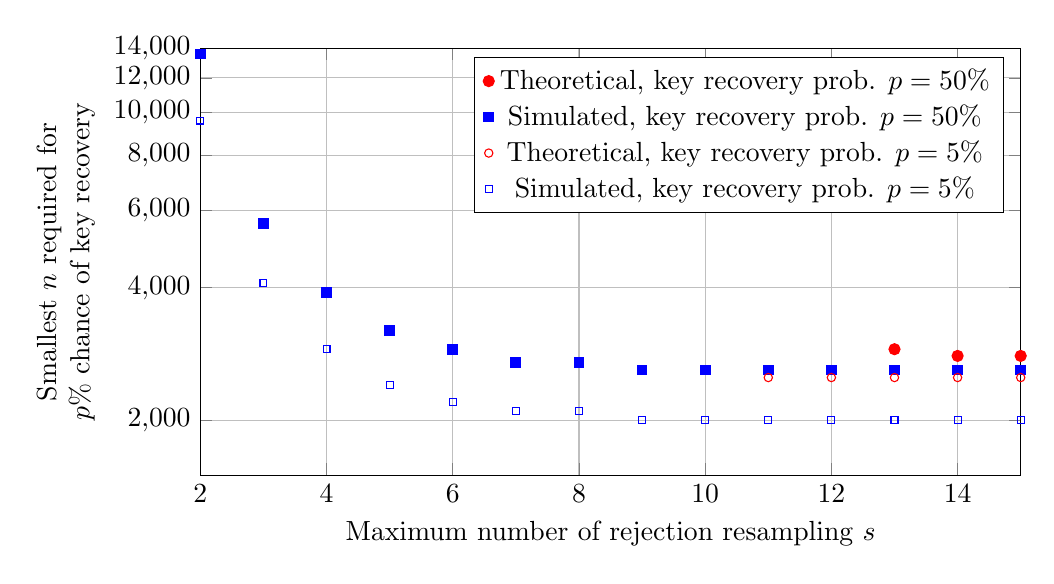
\begin{tikzpicture}
\begin{semilogyaxis}[
    enlargelimits=false,
    ymajorgrids=true,
    xmajorgrids=true,
    ymin=1500,
    ymax=14000,
    ytick={2000,4000,6000,8000,10000,12000,14000},
    log ticks with fixed point,
%    title={Key recovery parameter tradeoff},
    xlabel={Maximum number of rejection resampling $s$},
    ylabel={Smallest $n$ required for \\ $p$\% chance of key recovery},
    ylabel style={align=center},
    width=12cm,height=7cm
]
\addplot+[
    only marks,
    mark=*,
    color=red,
    mark options={fill=red},
    mark size=2pt]
coordinates{
(13,2900) (14,2800) (15,2800)
};
\addplot+[
    only marks,
    mark=square*,
    color=blue,
    mark options={fill=blue},
    mark size=1.75pt]
coordinates{
(2,13600) (3,5600) (4,3900) (5,3200) (6, 2900) (7, 2700) (8, 2700) (9, 2600) (10, 2600) (11, 2600) (12, 2600) (13, 2600) (14, 2600) (15, 2600)
};
\addplot+[
    only marks,
    mark=o,
    color=red,
    mark size=1.5pt]
coordinates{
(11,2500) (12,2500) (13,2500) (14,2500) (15,2500)
};
\addplot+[
    only marks,
    mark=square,
    color=blue,
    mark size=1.25pt]
coordinates{
(2,9600) (3,4100) (4,2900) (5,2400) (6,2200) (7,2100) (8,2100) (9,2000) (10,2000) (11,2000) (12,2000) (13,2000) (14,2000) (15,2000)
};
\legend{{Theoretical, key recovery prob. $p=50$\%},{Simulated, key recovery prob. $p=50$\%},{Theoretical, key recovery prob. $p=5$\%},{Simulated, key recovery prob. $p=5$\%}}
\end{semilogyaxis}
\end{tikzpicture}
\caption[Key recovery parameter tradeoff]{Key recovery parameter tradeoff, showing the smallest number of ciphertexts $n$ (rounded up to the nearest 100) that result in 50\% and 5\% probability of key recovery, for $\kappa$ of length 400, and the value of $s$ on the x-axis.}
\label{figure:kr_results}
\end{figure}

The main difference between the simulation values and the theoretical approximation comes from the requirement, in the theoretical case, that all attempts to encode key bits in ciphertexts must succeed. With small $s$, $(1-2^{-s})^n$ actually gets smaller as $n$ gets larger and dominates the key recovery estimation, whereas the key recovery probability should increase when more samples are collected. Directly calculating the complicated probability expression of key recovery without this assumption is precisely the difficulty that we are avoiding with the simulation.

Earlier, we noted that one of the advantages of this ASA over the ASA in \autoref{sec:asymASA} was better resilience to timing detection. Recall that the parameter $s$ determines the maximum number of regular encryptions that the subverted encryption algorithm will do to return one ciphertext. Effectively, the runtime of the subverted scheme is up to $s$ times the runtime of the unsubverted scheme. Knowing this, a large $s$ would allow a user to detect the ASA by timing the execution of the algorithm. We have shown that the ASA $\mathsf{ASub2}$ allows key recovery with $s=2$, which is the smallest value we can achieve with this acceptance-rejection framework.

While we haven't included timing attacks in our formalism, it is an important area of future work. Even with $s=2$, a timing attack would easily detect $\mathsf{ASub2}$. It is not clear if there is any way to modify these techniques to achieve a general ASA which is resistant to timing attacks. Indeed, a value of $s=1$ would be identical to unsubverted encryption, and there is no obvious way to implement a non-integer value of $s$. Perhaps an ASA based on acceptance-rejection techniques could have an expected value of $s$ lower than 2, and avoid detection by timing in this manner. Of the published ASAs we evaluated in \autoref{sec:statereset}, \cite{BSKC2019} and \cite{AC:CheHuaYun20} avoided timing detection by using an efficient ASA, where the execution time of the subverted algorithm is approximately the same as that of the unsubverted algorithm, but at the cost of making detectable use of state under state reset attacks. This therefore leaves a gap in the literature: are there ASAs which are undetectable under state resets \emph{and} timing attacks, using acceptance-rejection techniques or otherwise?

\subsection{Key recovery in the presence of state resets}
As for our type 1 ASA from \autoref{sec:asymASA}, regular state resets would reduce key recovery probability of the ASA in this chapter as it is currently written. However, in this case, it is possible to modify the scheme to maintain key recovery in the presence of state resets. Making $\textsf{PKE}$ deterministic effectively removes dependence of the ASA on any state at all, since the value of $\kappa$ can be recomputed without state (keeping state anyway would allow the ASA to do the work of recomputing $\kappa$ only when the state is reset, mitigating some of the inefficiency of this process). If the ASA does not require state, then key recovery works just as well during state resets as without them.

If \textsf{PKE} was deterministic, this would also allow for the possibility of shorter \textsf{PKE} ciphertexts. For example, Bellare, Boldyreva, and O'Neill provide a deterministic PKE scheme which conserves plaintext length. If $|\kappa|=|k|=128$, then key recovery would require fewer ciphertexts. For example, the simulated 50\% recovery values in \autoref{figure:kr_results} would converge to 700 instead of 2600.

Unfortunately, deterministic \textsf{PKE} causes difficulties for our security analysis in \autoref{sec:security}. \autoref{theorem:security} bounds the IND-CPA$'$ advantage against $\mathsf{ASub2}$ using the IND-CPA security of \textsf{PKE}, which would no longer be appropriate for a deterministic \textsf{PKE}. To address this, we would need to instead use security notions for deterministic \textsf{PKE}. Bellare et al. provide security notions for deterministic PKE under the condition of high-entropy plaintexts \cite{C:BelBolONe07}, which applies to our case ($k$ is the only plaintext encrypted, and is high-entropy). An analogue to \autoref{theorem:security} would need to be proven with this new security notion in order to prove that an ASA using deterministic PKE is a type 2 asymmetric ASA.
